\chapter{Design and Implementation}

This chapter provides details regarding the FMLearn application, implementation of the proposed concept, that is, Federated meta Learning and it's working mechanisms. Each component of the application is discussed in detail including the components that were considered and tested, but are not a part of the final experimentation. Explanation of all the design decisions are provided in detail so as it make it easier for the reader to understand how the application developed over-time and reached it's final state. The FMLearn application attempts to solve the issue of redundant work put in by developers to find the best algorithm and it's hyper-parameters repeatedly for a previously solved / optimised dataset and possibly suggesting algorithms for a previously unseen dataset as well. If this is achieved, the users of this application and the community in general will be greatly benefited by saving time spent waiting for program to complete, electricity consumed on the running the machines and cooling them, the computational power expended over a repetitive task and money spent in all of the above, to find the best algorithm and it's hyper-parameter.

The design and implementation choices led to the development of a working prototype of the concept Federated Meta-Learning and the application FMLearn. The server was developed in python and is used to portray the capabilities of the application. The concept of Federated Meta-Learning discussed in \ref{federated-meta-learning} and the changes in the workflow of a typical Machine Learning project caused due to the introduction of Federated Meta-Learning is discussed in section \ref{fml-workflow}. Then we discuss in detail the prototype FMLearn which was built to demonstrate this concept under section \ref{fmlearn}, while discussing it's architecture design in section \ref{architecture} along with some design decisions in section \ref{design-decisioins} and why these were taken. We will also be discussing in detail about the Model built by FMLearn to predict / recommend the potentially best algorithm(s) for a given task along with it's workflow. In section \ref{scikit-learn} we will be discussing in detail about the modifications made to scikit-learn so that it can act as a client to FMLearn along with discussing the data description used.

% \section{Requirements}

% \section{High-Level Overview}

\section{Federated Meta-Learning}
\label{federated-meta-learning}
Federated Meta-Learning focuses on learning algorithm performance measures for arbitrary tasks. Essentially federated meta learning is an ecosystem where the raw data is kept on the original devices and the meta data and performance metrics of the algorithm on the tasks would be stored on a central FML server. Using this historic performance data, predict the best performing algorithm along with its hyper-parameters for a previously seen or unseen task.

The input to Federated Meta-Learning is a description of the task, and the output is a recommendation for the potentially best performing algorithm(s) to solve that task. This recommendation could consist simply of a list of the best algorithms, or their predicted performance values. The list could also consist of multiple sub-lists created with different meta-learners.

In its simplest form, federated meta-learning would simply be a knowledge base or directory of algorithm-dataset performance measures. Ultimately, Federated Meta-Learning would be able to predict algorithm performance for unseen tasks.

\section{Workflow of Federated Meta-Learning}
\label{fml-workflow}

From section \ref{workflow-automl}, we know that a typical algorithm selection and configuration task using the AutoML tools result in a repetitive and time consuming process which in turn eats up a lot of computing resources, electricity and money. To tackle this problem Dr. Joeran Beel proposed Federated Meta-Learning as seen in section \ref{federated-meta-learning}. When we take this concept and apply it to the current ecosystem of Machine Learning tasks we get a workflow as show in Figure \ref{fml-workflow-diagram}.

\begin{figure}[t]
    \centering
    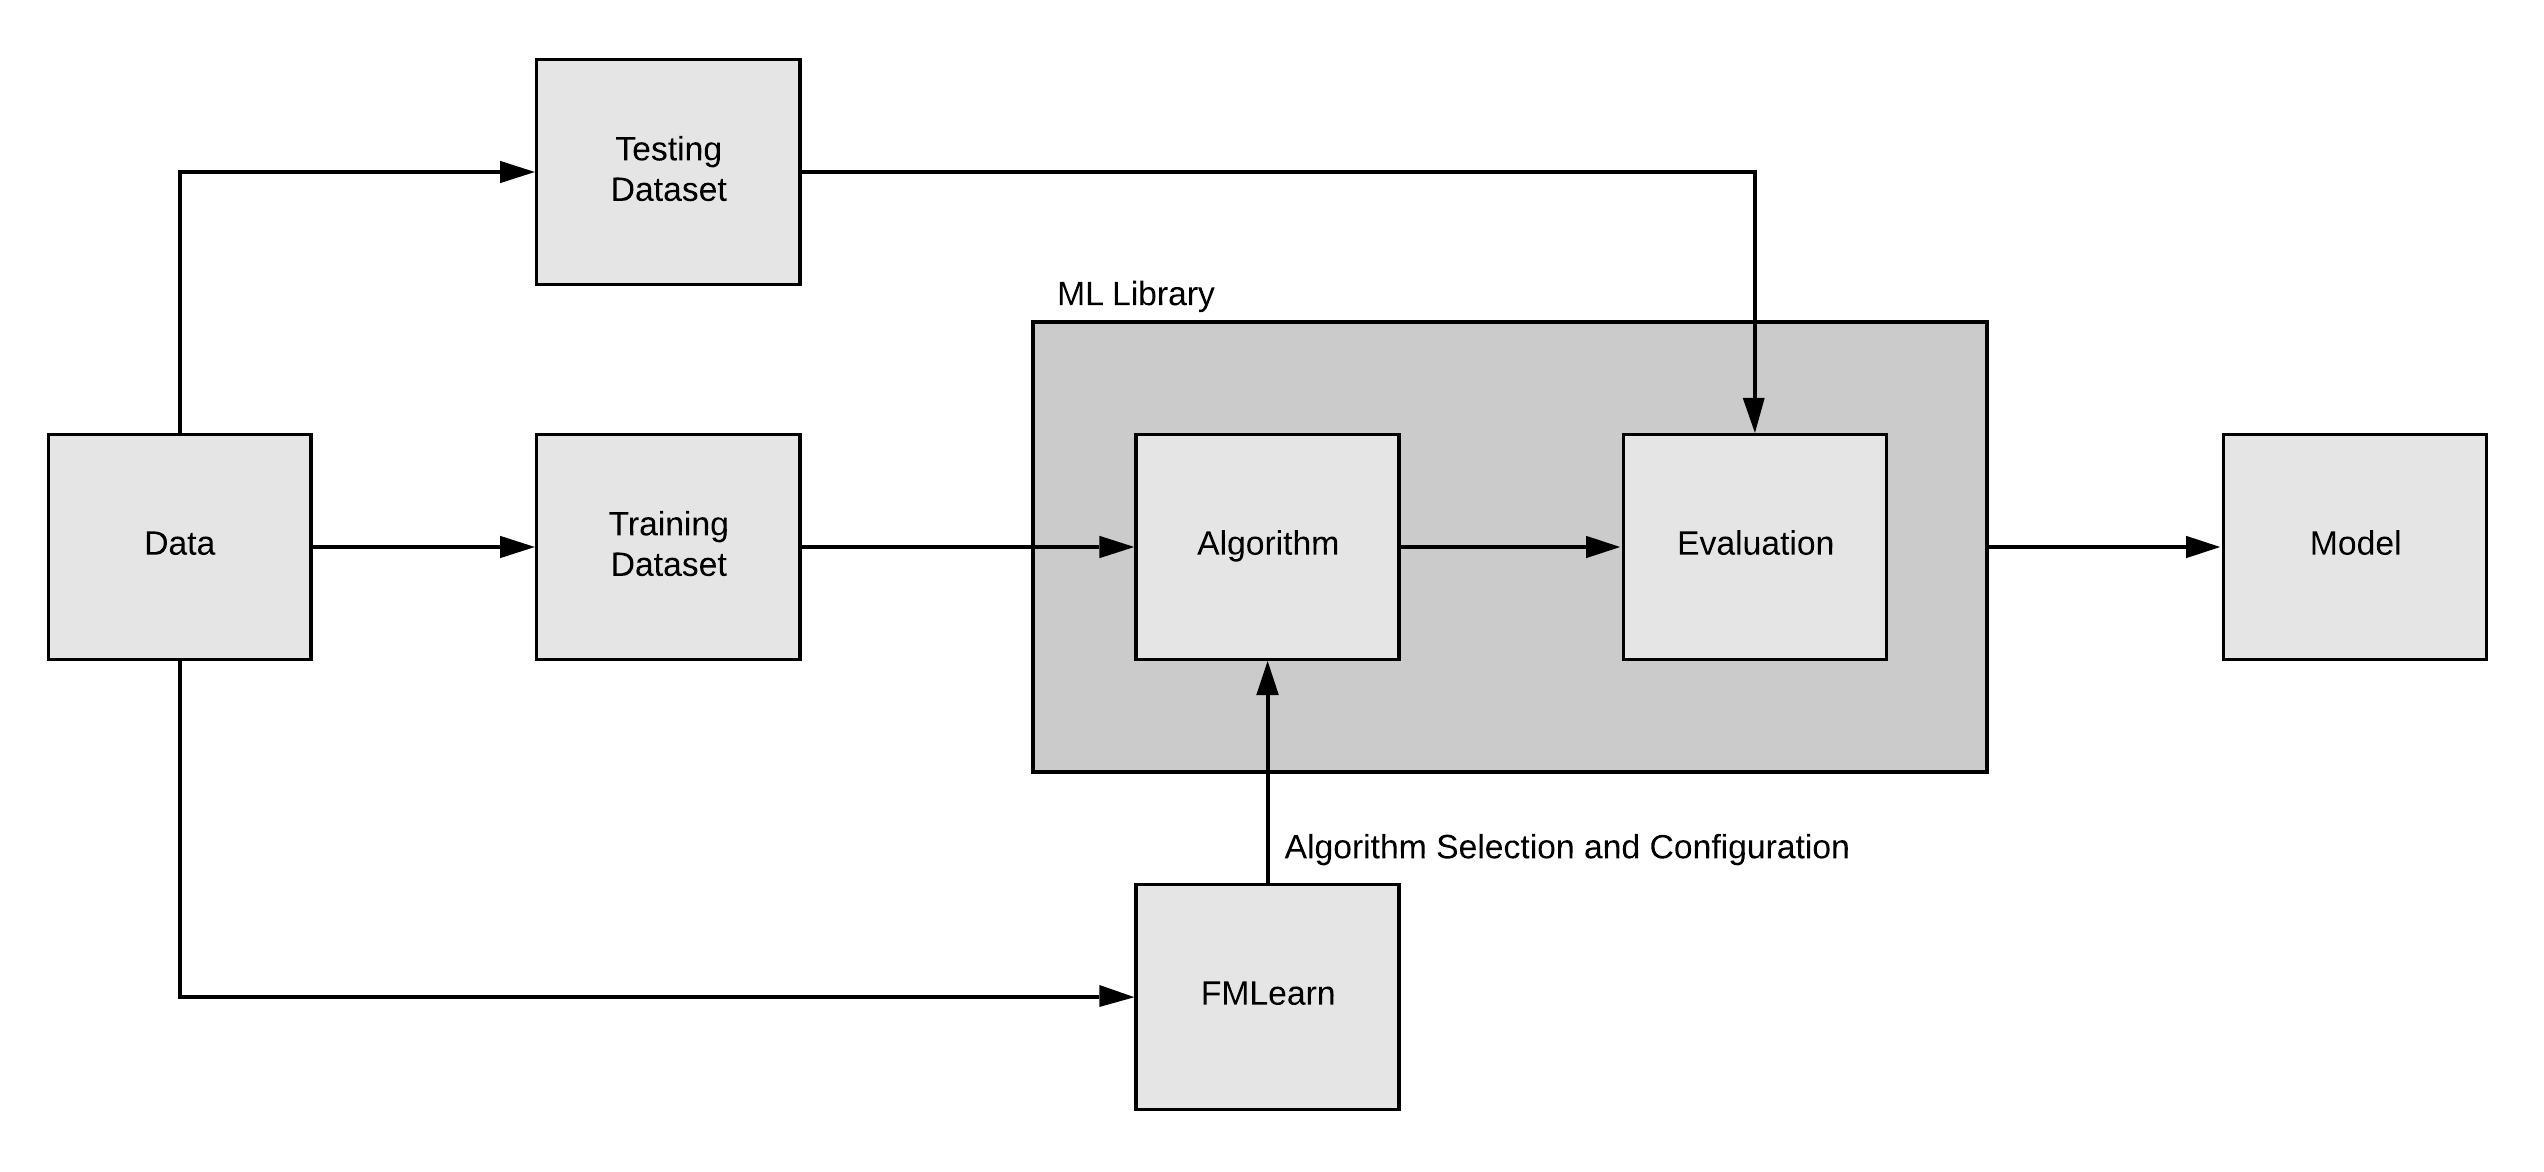
\includegraphics[width=15cm]{images/FML Workflow.jpeg}
    \caption{Federated Meta-Learning Workflow Diagram}
    \label{fml-workflow-diagram}
\end{figure}

Let's go into detail about the workflow of Federated Meta-Learning, Initial steps of the workflow remain similar to the working of AutoML (as seen in section \ref{workflow-automl}). The data is split into training and testing datasets, the training dataset in first sent to the library for the purpose of model creation. Here, the dataset is pre-processed using various techniques like data-cleaning, data imputation, data encoding, feature selection, feature exploration, feature engineering, feature co-relation, etc.

The difference between the 2 processes arise at the point when the data is obtained. The data apart from being sent to the library for pre-processing it is also sent to the Federated Meta-Learning application after finding the meta-features of the dataset. Once these meta-features are obtained Federated Meta-Learning predicts / recommends the potentially best performing algorithm(s) along with it's hyper-parameters for the given dataset. Once this recommendation is received by the Machine Learning library it re-optimises the algorithms and builds the model based on the training dataset which was received after pre-processing and this model is then evaluated against the testing dataset and then the final model is returned to the user.

The major difference with the workflows described in Figure \ref{automl-workflow-diagram} (as seen in the Section \ref{workflow-automl} - Workflow of AutoML Libraries) and Figure \ref{fml-workflow-diagram} is the introduction of an external application which applies the concept of Federated Meta-Learning. This application results in the elimination of the repetitive nature of algorithm selection and configuration task, which would drastically reduce the time spent on such a task along with the computational resources, electricity and money spent here.

\section{FMLearn}
\label{fmlearn}
FMLearn is an application which is a simple proof of concept of Federated Meta-Learning. FMLearn allows everyone to benefit from the data that is generated through machine learning and data science libraries. FMLearn is built using the Distributed Application Architecture (DAA), following the Client-Server Model. This allows the users to access as well as to exchange information and services with others. Though a Peer-To-Peer Model would be possible, this design was avoided due to the limitation in time as well as favouring the ease of development using the client-server model.

FMLearn consists of a client which is in our case a modified version of the popular Machine Learning library Scikit-Learn, but it could be any machine learning library and the Server is a Python Flask Application which handles all API calls and Data Store requests made by the user. FMLearn also acts as a knowledge base, storing all the algorithms-data performance measure collected though the machine learning library. The server also provides publicly available API's which can be accessed by any Machine Learning or Data Science tool to use FMLearn irrespective of the programming language used to build them to get a recommendation for the potentially best performing algorithm(s) and it’s hyper-parameters to solve it’s task without being constrained by the need to use the client that is supported by this paper (modified scikit-learn).

\subsection{Design Decisions}
\label{design-decisioins}
A few important Design Decisions that need to be addressed before proceeding with further discussions are as follows:
\begin{itemize}
    \item Why Client-Server Model?
    
    The biggest design decision was taken in the early stages of the dissertation. A decision was taken to proceed with the Client-Server model rather than a Peer-To-Peer model with respect to the architecture design of the application. This was an "Experience Based Design" as I have prior experience working with Client-Server Application model and more importantly due to the limited availability of time and ease of development which cannot be achieved / provided when following a Peer-To-Peer architecture.

    \item Why Scikit-Learn?
    
    Scikit-learn is a free software machine learning library for the Python programming language \citep{scikit-learn}. It is also among the popular and easy to use python libraries available in the market. Though other libraries with similar capabilities are available in the internet scikit-learn was chosen as an "Intuition Based Design" due to familiarity with the library and it's easy to use nature.
    
    \item Why a Public API Server?
    
    When Federated Meta-Learning was proposed by Dr. Joeran Beel \citep{fml}, he envisioned an ecosystem where everyone would benefit from the data that is generated though Machine Learning libraries and the prediction of the best performing algorithm along with it's hyper-parameters be available to all. A public API server ensures that even if the developers aren't using the supported client - modified scikit-learn - they can still benefit from the recommendations made by FMLearn.
    
    \item Why not a stand-alone client?
    
    A stand alone client was a possible aim for this dissertation, as the said client doesn't highly depend of the features provided by scikit-learn, though a few dependencies exists. But this idea was dropped due to limited availability of time and to concentrate on building and improving the server where the recommendations were to be made.
    
    \item Why Flask?
    
    Flask is a popular, extensible web micro-framework for building web applications with Python \citep{flask} and is among the most used web applications frameworks in python. It was a choice between Django and Flask, and Flask was chosen because of ease of use in terms of quick development when compared to Django. This was a "Reference Based Design" decision and when trying out both frameworks it was easier to get things started with Flask as opposed to Django. It is also easy to deploy Flask on to a free hosting services like Heroku, for the application to go live.
    
    \item Why PostgreSQL?
    
    PostgreSQL is a free and open-source relational database management system. It is easy to use when compared to other options and most importantly as it is a widely used database it was also available as a database deployment option in various online hosting platforms such as Heroku.
    
\end{itemize}

These are among the major design decisions made in the early stages of the dissertation which needed to be addressed before proceeding. Though other a few other design decisions were made during the process of development they will be explained as when we the appropriate section of the application is being explained.

\subsection{Architecture Design}
\label{architecture}

The figure \ref{architecture-diagram} describes the client-server architecture of the FMLearn application as a whole along with a few other components that haven't been discussed yet, these components will be introduced here and will be expanded upon later sections of this report. 

From the Figure \ref{architecture-diagram} we can see that the entire application is divided into two major chunks the client and the server. The client here is the modified version of Scikit-Learn which is explained in Section \ref{scikit-learn} in detail. To which I have introduced an additional package called `\texttt{fmlearn}`. This package provides the user with the capability to the interact with the server. This package also functions as an important link to the intermediary step where the data description is obtained for a given dataset or task i.e., the dataset is converted into it's meta-features. The conversion of dataset to it's Meta-Features is handled by a 3rd party library called Auto-Sklearn \citep{feurer:m}. Auto-Sklearn is an external library and a dependency introduced here details about which will be further explained in Section \ref{auto-sklearn}.

\begin{figure}[t]
    \centering
    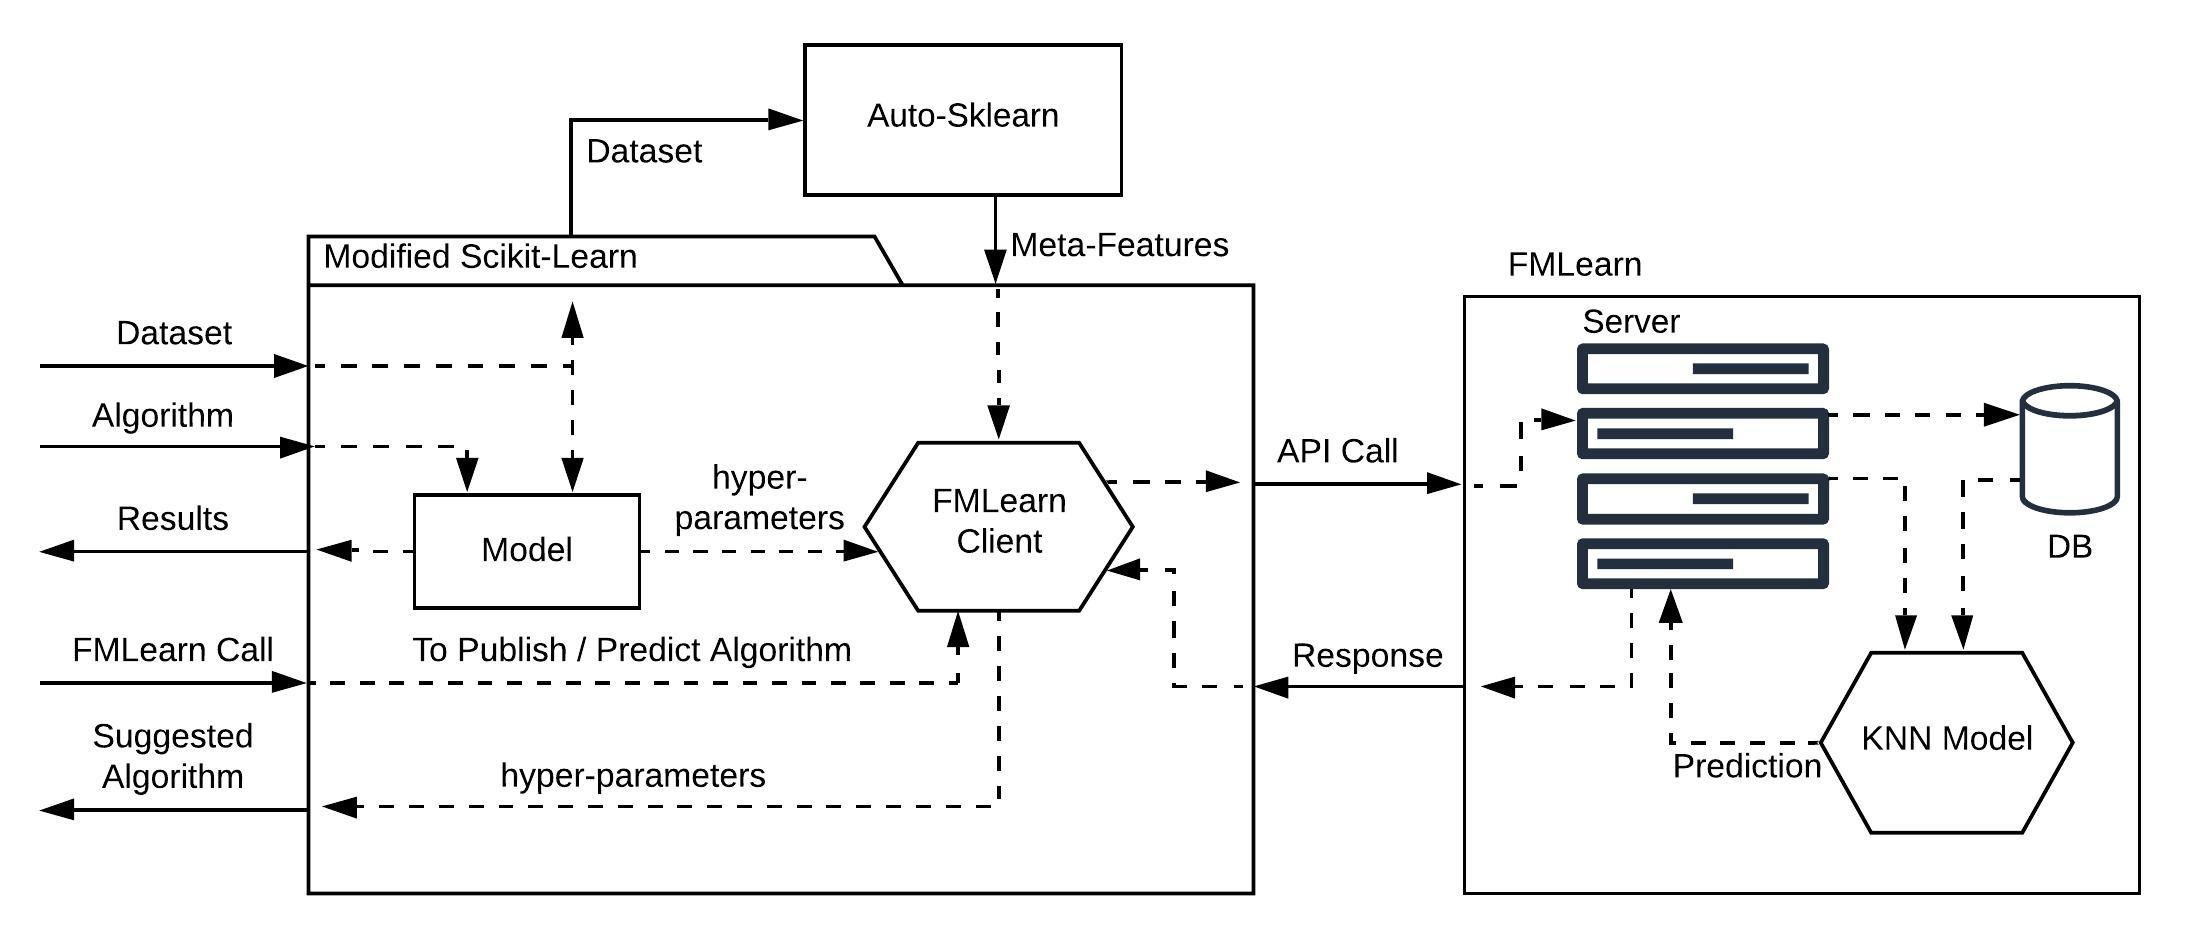
\includegraphics[width=15cm]{images/FML Architecture Diagram.jpeg}
    \caption{Architecture Diagram}
    \label{architecture-diagram}
\end{figure}

The client majorly performs 2 tasks, publishing the data to the server and displaying the results obtained for algorithm recommendation from the server to the user. Irrespective of the task, the \texttt{fmlearn} module obtains the dataset from the user and it is converted to it's Meta-Features with the help of Auto-Sklearn. Depending on the task the user might want a recommendation of the best performing algorithm or might want to contribute his findings to the betterment of the FMLearn in general. Depending on the use case either an API call is made to obtain the recommendation for the user or the model details along with the performance metrics is obtained from the user and the model directly and then an API call is made to publish these details to the server respectively.

The server performs various roles depending on the task and is explained in Section \ref{fmlearn-server} in detail. The server primarily acts a recommender system, recommending algorithm(s) for a given task. The server also acts a knowledge base or directory of algorithm-dataset performance measures, apart from this is also provides API's to expand or build this knowledge base. This knowledge base is stored in a PostgreSQL Database and it also used to build a Machine Learning model, The model was built using the K-Nearest Neighbors algorithm. The details about the model and algorithm in general will be discussed in the Section \ref{knn-model}. This model is used to make recommendations to the users for previously seen or unseen task or dataset. The model's ability to recommend the best performing algorithm(s) have been exposed to the public via API's.


\section{The Client: modified Scikit-Learn}
\label{scikit-learn}

In this Client-Server Architecture, the stable release of the client i.e., modified version of scikit-learn is available on GitHub via the following link:
\begin{center}
\href{https://github.com/mukeshmk/scikit-learn/releases/latest}
{\texttt{https://github.com/mukeshmk/scikit-learn/releases/latest}}.
\end{center}

The complete code repository is available at: \href{https://github.com/mukeshmk/scikit-learn/}{\texttt{https://github.com/mukeshmk/scikit-learn/}} \newline which is forked from: \href{https://github.com/scikit-learn/scikit-learn}{\texttt{https://github.com/scikit-learn/scikit-learn}}.

After downloading the stable release and installing the library by following the instructions specified in the \texttt{README.md} file, we can use it normally as we use scikit-learn, since it's a fork of the original release it has all the features of the stable release plus it has the features of FMLearn.

To initialise \texttt{fmlearn}'s client we have to import the \texttt{FMLClient} package from \texttt{sklearn.fmlearn} and then create an object of the class \texttt{FMLClient} as follows:
\begin{lstlisting}
    # imports the FMLearn client into the program
    from sklearn.fmlearn import FMLClient
    # initialises the client
    fmlearn = FMLClient()
\end{lstlisting}

Once the client as been initialised irrespective of the task the first thing to do would be do tell \texttt{FMLearn} what dataset we will be using for the task this can be done as follows:

\begin{lstlisting}
    # assuming that the import for train_test_split has been done
    # and the data has been loaded and split into 'X' and 'y'
    x_train, x_test, y_train, y_test = train_test_split(X, y, test_size=0.2, random_state=12)

    # this is a function introduced by the Client to let FMLearn know 
    # what dataset is being used for the task.
    fmlearn.set_dataset(x_train, y_train, x_test, y_test)
\end{lstlisting}

Setting the dataset using the \texttt{sets\_dataset()} method triggers a background call to an external 3rd party library called Auto-Sklearn which is used to describe the Dataset and obtain the Meta-Features for that dataset. This is further explained in Section \ref{auto-sklearn}. These Meta-Features thus collected is then sent to the server to be processed as required.

Depending on the objective of the user, the user can proceed with the program in one of these two ways:
\begin{enumerate}
    \item Get recommendation for a task.
    \item Publish performance data for a task.
\end{enumerate}
If the user wants to get a recommendation for a task all they would have to do this to calls the methods \texttt{predict\_metric()} as follows.

\begin{lstlisting}
    # this method returns the recommendation of the
    # best performing algorithm along with its hyper-parameters
    # for the dataset set using the set_dataset() method
    fmlearn.predict_metric()
\end{lstlisting}

This method provided by the client internally makes an API call to the server sending the server the Meta-Features of the dataset which was obtained from \texttt{auto-sklearn}. Upon reaching the server, the server processes the request, responding with the appropriate algorithm recommendation which is then sent to the user as shown in Figure \ref{sample-output}. The recommendation can then be used by the user to create a model with the specified algorithm and the hyper-parameter values. The created model can then be used by user to proceed with the task after re-optimising the parameters to suite the users dataset.

\begin{figure}[H]
    \centering
    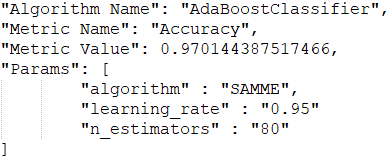
\includegraphics[width=9cm]{images/sample-output.png}
    \caption{Sample Output}
    \label{sample-output}
\end{figure}

If the user wants to publish a performance metric for a task which they performed, the user can do so by using the \texttt{publish()} method by passing the model used, scoring metric and the score as it's parameters as follows:

\begin{lstlisting}
    # the `model` parameter contains the model trained using the dataset
    # `fmlearn.ACCURACY` specifies the evaluation metric used
    # the `score` parameter contains the evaluation results.
    fmlearn.publish(model, fmlearn.ACCURACY, score)
\end{lstlisting}

Upon calling the client's \texttt{publish} method the meta-features of the dataset, model details including the algorithm name, hyper-parameters, along with the evaluation metric and the evaluation scores are sent to the FMLearn server. This data is processed and stored in the database, which is later be used to build a model.

\subsection{Data Description: Auto-Sklearn}
\label{auto-sklearn}

Auto-sklearn \citep{feurer:m} is an open-source AutoML tool written in Python that automatically determines effective machine learning pipelines for classification and regression datasets. Though this is an AutoML tool, it was used here for it's \textbf{meta-learning} step in the AutoML pipeline, which it uses to warm start the Bayesian optimization procedure in it's core. This meta-learning step is abstracted inside all the features provided by the tool and is not easily available to the users to use outside the tool.

An utility package was introduced inside the FMLearn's client (modified Scikit-Learn) to make use of the meta-learning feature provided by auto-sklearn. This utility function performs the input checks, transforms the data and performs the required validations before passing on the dataframe to Auto-Sklearn's calculate meta-features method. It is available in this package via the imported method.

\begin{lstlisting}
            from autosklearn.metalearning.metafeatures.metafeatures 
            import calculate_all_metafeatures_with_labels
\end{lstlisting}

The input to the \texttt{calculate\_all\_metafeatures\_with\_labels()} method is the dataset and the output is a set of meta-features. These meta-features are then converted into the required format and then forwarded to server via API calls. A few of the meta-features thus obtained are: \texttt{ClassEntropy, ClassProbabilityMean, NumberOfMissingValues, NumberOfCategoricalFeatures, NumberOfNumericFeatures, etc}. Depending on the dataset there can be about 24-30 meta-features obtained for a given dataset. For the complete list of meta-features and to see a few examples of values obtained via the Auto-Sklearn took please refer Appendix \ref{meta-features-ask}. The end user is abstracted away from existence of this feature, the call to auto-sklearn is handled internally by the client upon letting the client know about the dataset in use.

\begin{lstlisting}
    # this is a method provided by the FMLearn client that internally calls
    # `calculate_all_metafeatures_with_labels()` method provided by auto-sklearn
    # which provides the meta-features required.
    fmlearn.set_dataset(x_train, y_train, x_test, y_test)
\end{lstlisting}

Before finalising with \texttt{auto-sklearn} another library by Hadi called \texttt{dataset2vec} \citep{dataset2vec} was explored and evaluated for it's effectiveness in model building. This library represents a tabular dataset in a hierarchical fashion by defining a dataset as a set of features, where each feature is a set of instance values. Working with this library proved to be quite challenging due to the lack of documentation and lack of pre-trained model which converts the dataset to it's meta-features and thus making it necessary for the user to train a model. Though this paper claimed to out-perform the current state-of-the-art, a design decision was made to not use \texttt{dataset2vec} and instead proceed with \texttt{auto-sklearn} as a model was available and also a support by the community to improve the meta-feature extraction model.

\section{The Server: FMLearn}
\label{fmlearn-server}

The stable release of the server - FMLearn in this Client-Server Architecture is available on GitHub via the following link:

\begin{center}
\href{https://github.com/mukeshmk/fm-learn/releases/latest}
{\texttt{https://github.com/mukeshmk/fm-learn/releases/latest}}.
\end{center}

The complete code repository is availabe at: \href{https://github.com/mukeshmk/fm-learn}{https://github.com/mukeshmk/fm-learn}. The application is also deployed on Heroku. Heroku is a platform as a service (PaaS) that enables FMLearn to available on the cloud to be accessed by everyone. The application is deployed and available via the link mentioned below, though this is an API server a basic user-interface has been developed so as to provide information about Federated Meta-Learning and API documentation.

\begin{center}
\href{https://fmlearn.herokuapp.com/}
{\texttt{https://fmlearn.herokuapp.com/}}.
\end{center}

The server provides several API's among which two of the important API's are the \texttt{publish} and \texttt{predict} API's. These API's represent the two important functionalities of the proposed prototype. 

The \texttt{publish} API solves the problem with the workflow of machine learning and data science libraries. These libraries usually work in isolation and the information regarding how an algorithm performs on a particular dataset is neither publisher nor shared. The publish API can be called from within these libraries as done in the modified scikit-learn presented and thus enabling the users to share the algorithm performance data. The API is a \texttt{POST} method which can be accessed via this endpoint \texttt{/metric} and takes a JSON object as input in this format:

\begin{lstlisting}
# the input JSON object to publish API
{
	"algorithm_name": algorithm_name,
	"dataset_hash": dataset_hash,
	"meta_features": [
		{
			"feat_name": feature_name,
			"feat_value": feature_value
		}
	],
	"metric_name": metric_name,
	"metric_value": metric_value,
	"params": [
		{
			"param_name": hyper_parameter_name,
			"param_value": hyper_parameter_value
		}
	],
	"target_type": target_type
}
# NOTE: "meta_features and params" are a list of objects
# but for illustration purpose only 1 item has been shown.
\end{lstlisting}

This data is validated, preprocessed and stored in the database. A PostgreSQL database used in this application which contains 3 tables to store the information received from the client. These tables are structured as follows as shown in Figure \ref{class-diagram}. The three tables are \texttt{Metric}, \texttt{Meta Feature} and \texttt{Params}, the \texttt{Metric} table has a one to many relation ship with both the \texttt{Meta Feature} and \texttt{Params} tables and this relationship puts the database in it's 3rd Normal Form.

\begin{figure}[H]
    \centering
    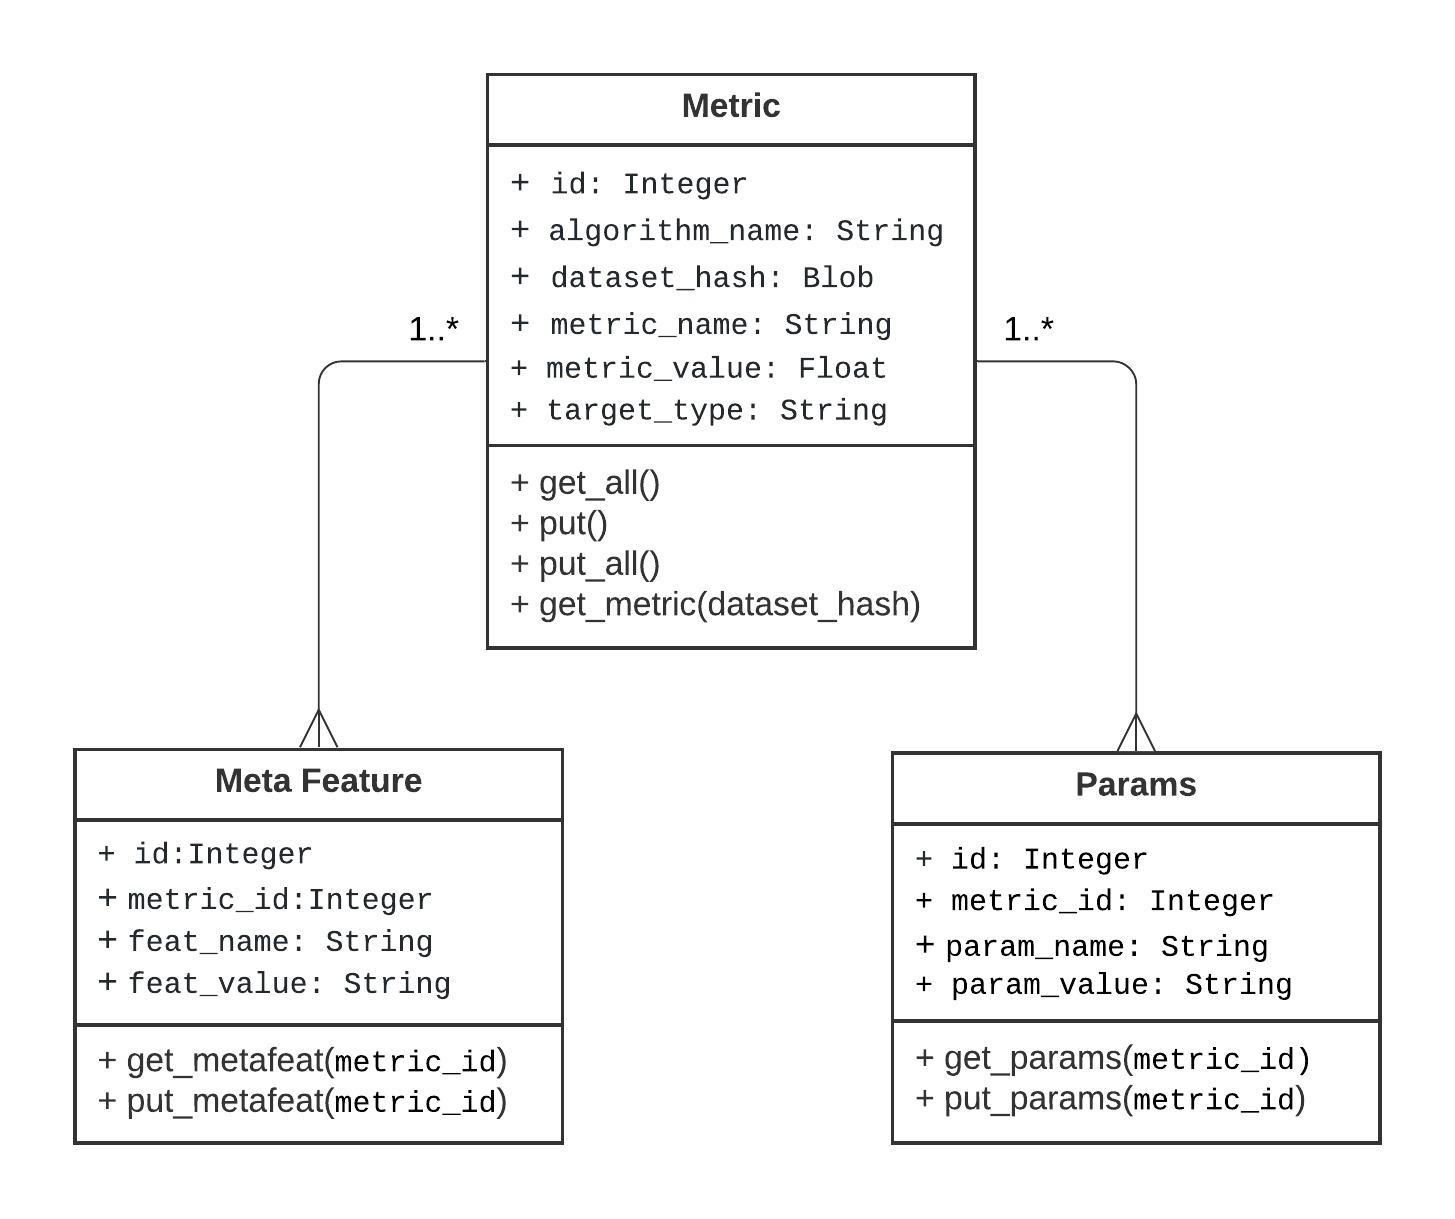
\includegraphics[width=15cm]{images/Class Diagram.jpeg}
    \caption{Class Diagram}
    \label{class-diagram}
\end{figure}

This database thus created acts as a knowledge base which contains information about the algorithm-data performance metrics. FMLearn also provides others API's to access this data which enables sharing of performance details of various algorithms among software libraries. The response of this API when there are no internal errors is a JSON object similar to the request object with a HTTP status code of 200.

The \texttt{predict} API solves the problem with the repetitive nature of the workflow of machine learning libraries, where the algorithm selection and hyper-parameter optimization tasks have to been done repeatedly. The \texttt{predict} API can be called by the machine learning libraries as done in the modified scikit-learn presented in this paper and thus breaking the cycle and saving time, electricity, computation power and money. The API is a \texttt{GET} method which can be accessed via this endpoint \texttt{/metric/predict} and the API accepts a JSON object as input which is similar to the below format:

\begin{lstlisting}
# the input JSON object to predict API
{
	"dataset_hash": dataset_hash,
	"meta_features": [
		{
			"feat_name": feature_name,
			"feat_value": feature_value
		}
	],
	"target_type": target_type
}
# NOTE: the key "meta_features" accepts a list of objects
# but for illustration purpose only 1 item has been shown.
\end{lstlisting}

This input is validated, preprocessed and then sent to the model for the best algorithm prediction (this is discussed in detail in Section \ref{knn-model}) and the result of the prediction is sent to the user as the best algorithm recommendation for the given task. This response is a JSON object in the following format:

\begin{lstlisting}
# the output JSON object of predict API
{
  "recommendations": [
    {
      "algorithm_name": algorithm_name,
      "metric_name": metric_name,
      "metric_value": metric_value,
      "params": [
        {
          "param_name": hyper_parameter_name,
          "param_value": hyper_parameter_value
        }
      ],
      "target_type": target_type
    }
  ]
}
# NOTE: "recommendations and params" are a list of objects
# but for illustration purpose only 1 item has been shown.
\end{lstlisting}

\subsection{KNN Algorithm}
\label{knn-model}

The goal is to use FMLearn to try and find the closest existing dataset which is very similar to the dataset for which an algorithm is to be recommended. Then recommend the best performing algorithm for the requested dataset based on the existing data. I am not trying to predict the best performing algorithm, this is an important point to be noted in the algorithm recommendation process. Prediction of an algorithm using a model might not be feasible as there are various types of algorithms classification, regression and clustering just to name a few and various algorithms within each type of problem, various performances and on top of this it will be a multi-class output problem. This problem will be trying to predict algorithm name, metric used, metric value, and not to mention the parameters of an algorithm. This will result in a lot of mismatch in the output making the prediction a random set of values. Thus predicting the closest existing dataset for the input dataset and then finding the best algorithm for that dataset is the best possible approach in the scenario.

The algorithm used to predict or recommend the best performing algorithm for a given task is the \textbf{K-Nearest Neighbours (KNN)} algorithm. KNN is a supervised, non parametric learning algorithm, meaning, the target variable is known and that it does not make an assumption about the underlying data distribution pattern. In the case of FMLearn, a KNN classification algorithm has been used with k=1 and the distance between points is calculated using Euclidean distance. The "K" in KNN is the number of nearest neighbors considered before labeling the current point or in terms of FMLearn number of datasets that has 

\subsection{Model Building}
\label{model-building}


\section{The Big Picture}



\begin{figure}[H]
    \centering
    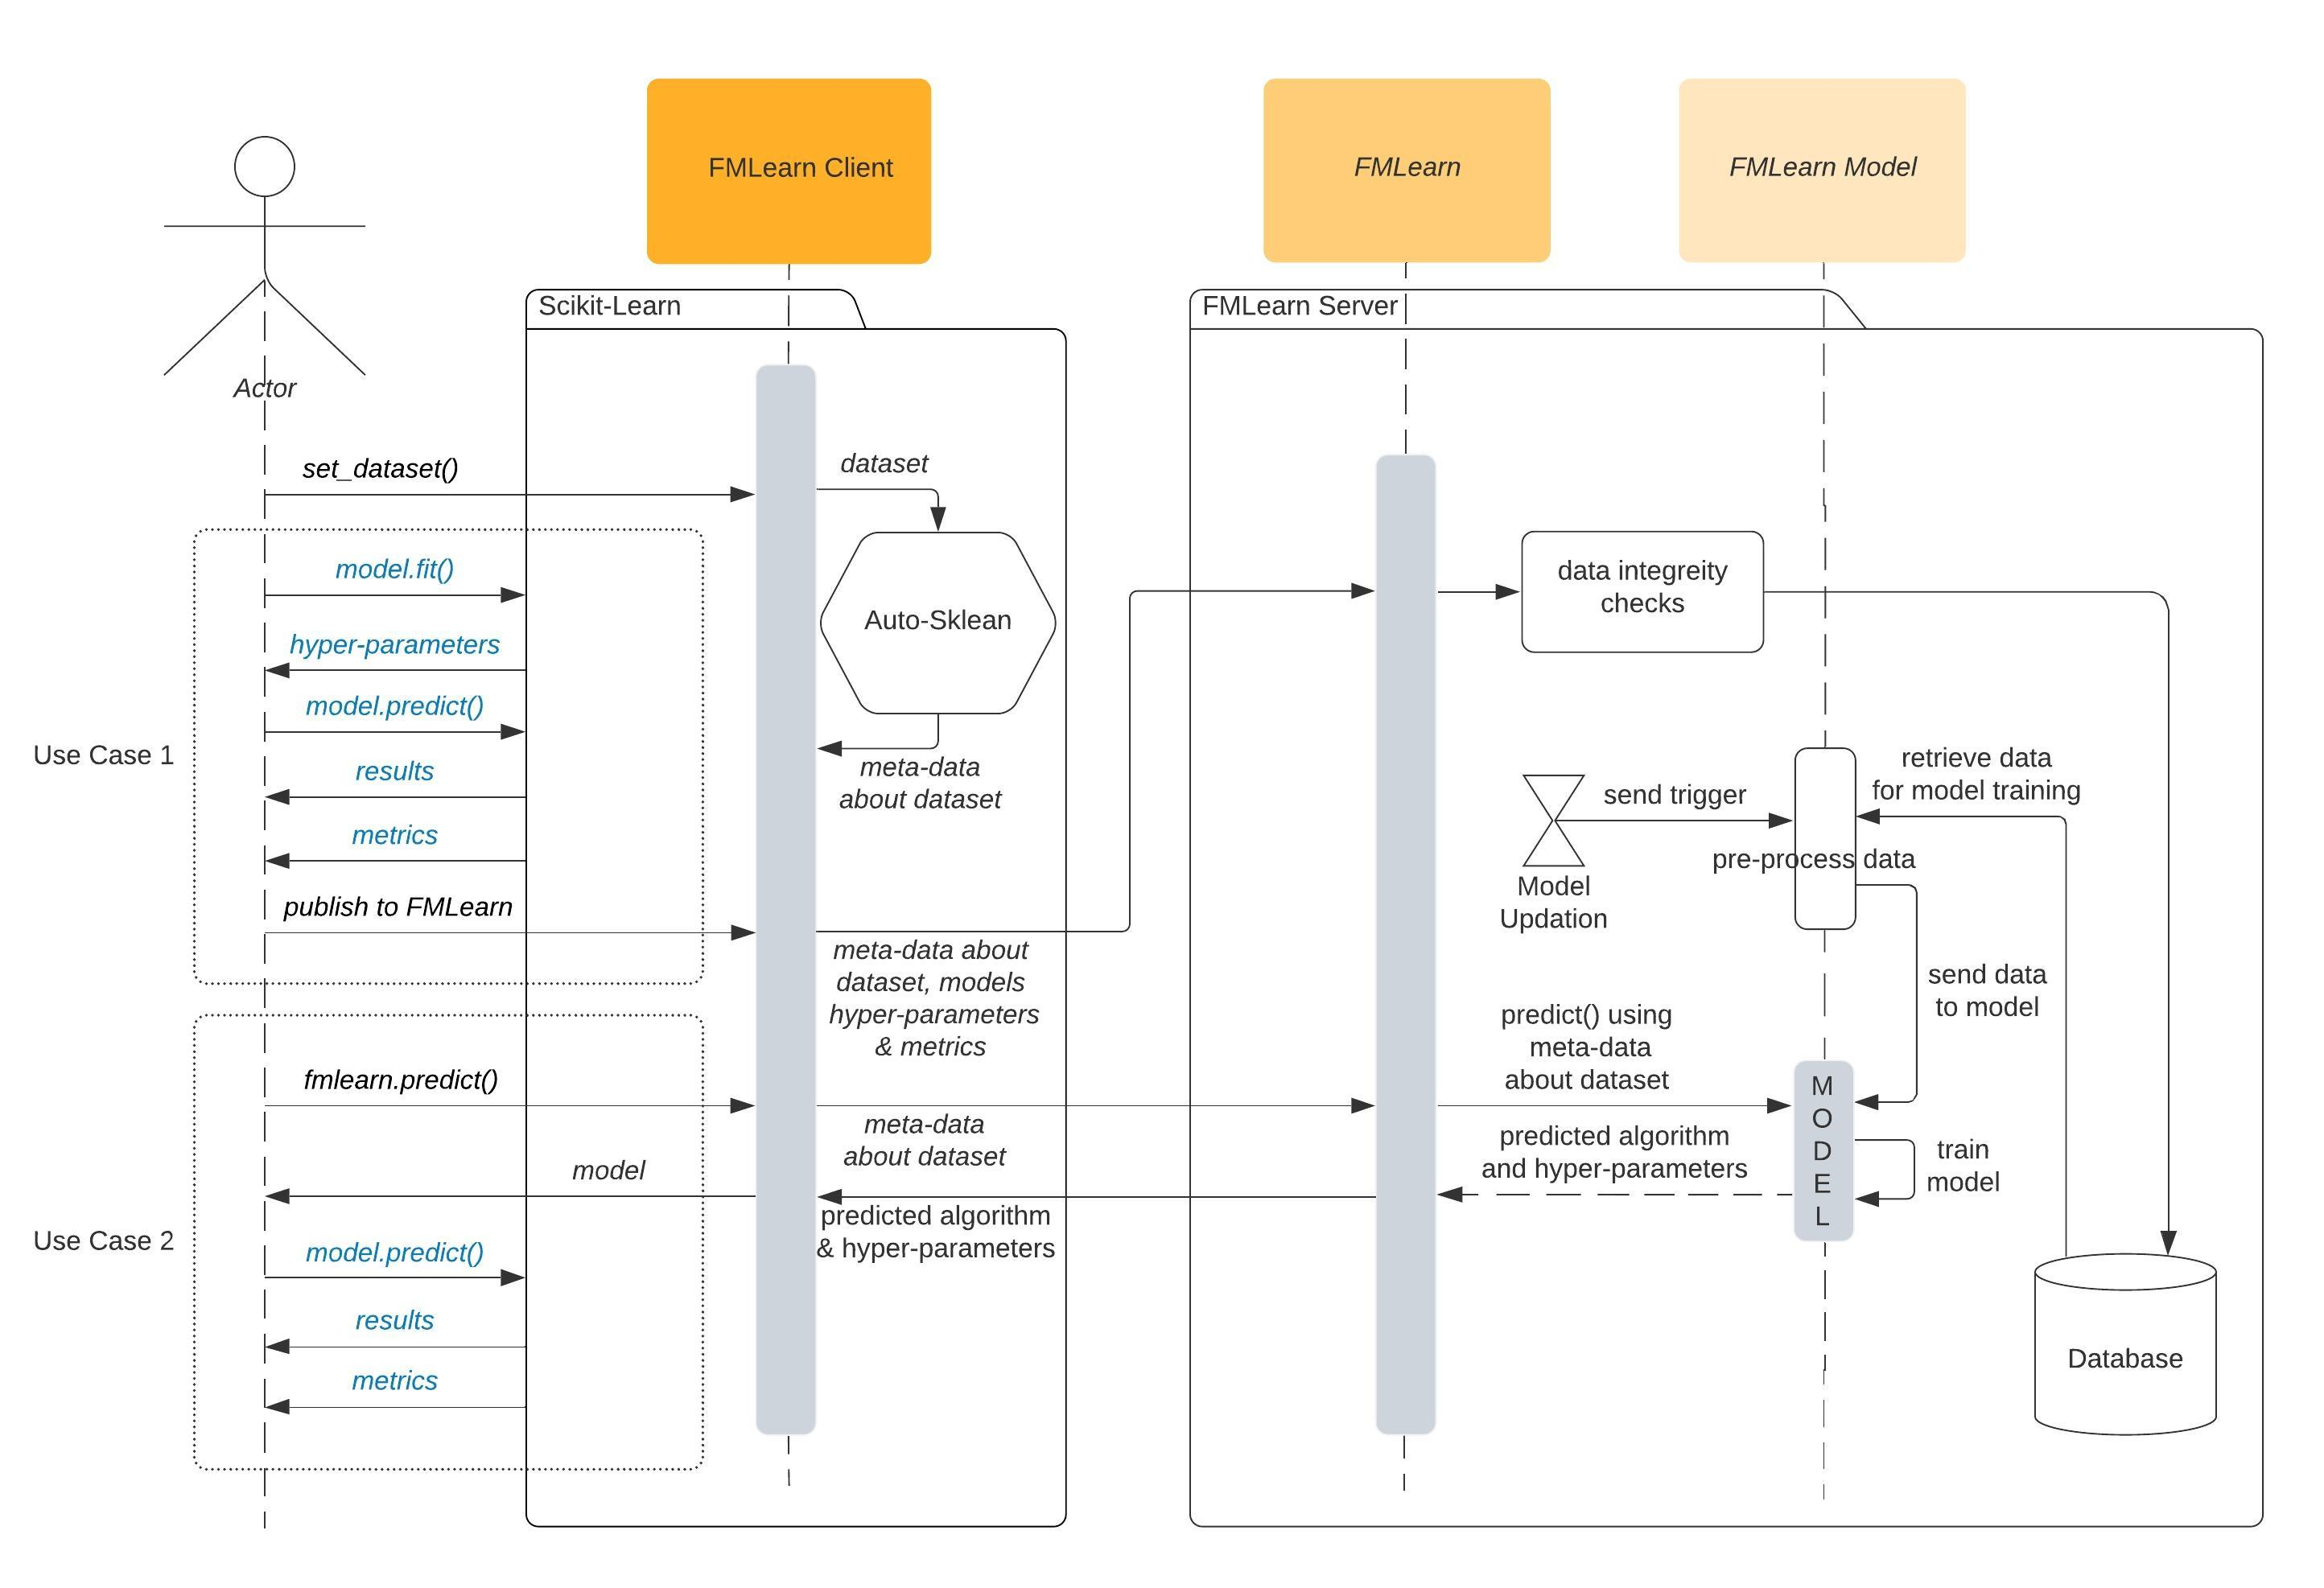
\includegraphics[width=15cm]{images/Sequence Diagram.jpeg}
    \caption{Sequence Diagram}
    \label{sequence-diagram}
\end{figure}


\section{Security and Privacy Concerns}
FMLearn is a client-server architecture-based [2] application which provides public API’s for it's users, and it brings its own security and privacy concerns. The different aspects of security and privacy issues that are to be considered with respect to FMLearn are - but not limited to:

\begin{enumerate}
    \item A client-server architecture.
    \item Publicly available API server [3] (which could be broken down)
\end{enumerate}

\subsection{Security Concerns}

FMLearn was built using Python Flask, and uses PostgreSQL, which acts as the public API server which exposes various API to users to use the application and is currently hosted on Heroku .

One of the most important security concerns with the current implementation of FMLearn is that the users have unlimited access to APIs (Flash Crowd Problem) [4], this could have severe consequences. A denial of service is possible, and extraction of all information of few of the major effects. This could be resolved using various rate-limiting strategies:

\begin{itemize} 
    \item Limiting per connection property (IP address)
    \item Limiting per user (account / access token / API key)
    \item Limiting per application property (user account / resource type)
    \item Limiting based on context (region / type of app)
\end{itemize}

Once these rate-limiting features have been introduced if someone tried to repeatedly access the API, they would get the following error.

\quad\quad\quad\quad\quad\quad\quad\quad\quad\quad\quad\quad\quad
\texttt{HTTP/1.1 429 Too Many Requests}\\
\quad\quad\quad\quad\quad\quad\quad\quad\quad\quad\quad\quad\quad
\texttt{Retry-After: 3600}


Rate limiting prevents malicious code from abusing legitimate / illegitimate access to the API.

One of the basic and yet most powerful technique which helps prevent a lot of security issues is Input validation [5]. Input validation should act as the first line of defense in case of a malicious attack. It is also useful to reject malicious data which helps prevent DoS attacks by rejecting unreasonably large inputs and against injection attacks by rejecting crafted payloads. Some of the possible Input validation techniques which could be easily enforced in my case are:

\begin{itemize}
    \item Enforcing sensible length limits on inputs.\\
    (i.e., 2MB of user’s hashed dataset is not allowed)
    \item Enforcing strict content types on provided data inputs.\\
    (i.e., an API expecting JSON data should not accept anything else.
    \item Enforcing strict data type checking on inputs.\\
    (i.e., Numbers should be numbers, and SQL code as input results in an error)
\end{itemize}

Even though input validation is a decent first line of defense, it will fail if used as the only line of defense because when the application evolves and brings in complex input types it will not prevent attacks as it will be complex to determine the validity of complex data at input time. Moreover, complex validation procedures usually suffer from bypass attacks, and making validations might break functionality. [6]

\subsection{Data Protection}
Another possible issues specific to FMLearn is the storage of hash for the complete dataset in the proposed prototype, the dataset is hashed using sha256 though this is very secure it has its own set of vulnerabilities [7] that need to be taken into consideration, for now we can assume that sha256 is safe to use. But if it is broken there is a possibility that all the user data can become compromised. Even if the hash of the dataset is not broken, but if the meta-data about the model (like the model parameters) and dataset is available to the hacker, it is very much possible that a model could be reconstructed and the data of the user can be compromised.

Currently FMLearn is also vulnerable to Eavesdropping Attack, this is because the data sent from scikit-learn to FMLearn is not encrypted and is in plain-text, so various sniffing tools like Wireshark, Nmap, etc., can be used to monitor the network traffic and sniff the data transmitted between client and the server. To prevent such attacks, I can use a technique similar to twitter’s developer API access, where in the user is required to create an account with FMLearn and is required to use certain keys generated during account creation:

\quad\quad\quad\quad\quad\quad\quad\quad\quad\quad\quad\quad\quad\quad
\texttt{ACCESS\_TOKEN = ''\\}
\quad\quad\quad\quad\quad\quad\quad\quad\quad\quad\quad\quad\quad\quad
\texttt{ACCESS\_TOKEN\_SECRET = ''\\}
\quad\quad\quad\quad\quad\quad\quad\quad\quad\quad\quad\quad\quad\quad
\texttt{API\_KEY = ''\\}
\quad\quad\quad\quad\quad\quad\quad\quad\quad\quad\quad\quad\quad\quad
\texttt{API\_SECRET\_KEY = ''}

This introduces a 3-legged oauth authentication workflow similar to twitter’s developer API [8] access and these tokens can them be used to securely transfer data back and forth between the client and server, without worrying about eavesdropping attack. But then by introducing this we bring in new security vulnerabilities into the application which needs to be addressed separately in a larger scale. But for now sticking to just encrypting the information related to dataset let it be dataset hash or meta-data about the data, can be done as the first step in the necessary direction for this dissertation to proceed using public key encryption techniques. Doing just this helps protect the privacy of the user’s data from potential sniffers and maintains the integrity of the data over the network.

The scope of improvement in terms of security is huge in this project, it can be made secure enough for users to confidently use, but all this is just until things don’t go wrong.

\subsection{Social Concerns}
In the long run, social questions need consideration such as preventing manipulation (developers of algorithms may have an interest that their algorithms are "recommended") and free-rider problems (users benefiting from the system without sharing their data).

